\documentclass{beamer}
%%%%%% UNOFFICIAL ICL BEAMER TEMPLATE V.0.1 %%%%%%
% This is a basic LaTeX Beamer template that I customised to have the logo of ICL and a background picture. Mind that this is NOT an official ICL template but it may still be useful for informal presentations.
% The official ICL graphical identity resources can be found here: http://www3.imperial.ac.uk/graphicidentity
% Please drop me an e-mail or comment via Twitter @AJunyentFerre if you found this was useful or have any suggestion to improve it.
%%%%%%

\usepackage[english]{babel}
\usepackage{xcolor}
\usepackage{xmpmulti}
\usepackage{amsmath}
\usepackage{eucal}
\usepackage{tikz}
\usepackage{url}
\usepackage{graphicx}
\usepackage{dsfont}

\usepackage{pgfplots}
\usepgfplotslibrary{groupplots}
\usetikzlibrary{pgfplots.groupplots,arrows.meta,shadows,positioning,angles,quotes}
\usetikzlibrary{matrix,chains,positioning,decorations.pathreplacing,arrows}
\usepackage{tikz}
\usetikzlibrary{shapes.geometric}
\usetikzlibrary{positioning}

\usepgfplotslibrary{fillbetween}


\DeclareMathOperator*{\argmax}{arg\,max}
\def\checkmark{\tikz\fill[scale=0.4](0,.35) -- (.25,0) -- (1,.7) -- (.25,.15) -- cycle;} 
\definecolor{webgreen}{rgb}{0,.5,0}
\definecolor{webbrown}{rgb}{.6,0,0}
\definecolor{Maroon}{cmyk}{0, 0.87, 0.68, 0.32}
\definecolor{RoyalBlue}{cmyk}{1, 0.50, 0, 0}
\definecolor{Black}{cmyk}{0, 0, 0, 0}
\definecolor{skymagenta}{rgb}{0.81, 0.44, 0.69}

%%%%%% THE FOLLOWING FILE CONTAINS THE STYLE DEFINITIONS %%%%%%
\usepackage[utf8]{inputenc}
\usepackage[export]{adjustbox}

\definecolor{gris}{rgb}{0.92,0.92,0.92}
\definecolor{blau-upc}{rgb}{.192,.365,.506}

\setbeamercolor{titlelike}{fg=blau-upc}
% \setbeamercolor{barra}{bg=white,fg=white}
\setbeamercolor{capcalera}{bg=blau-upc,fg=white}
\setbeamercolor{section in toc}{fg=blau-upc}
\setbeamertemplate{sections/subsections in toc}[circle]
\setbeamertemplate{itemize items}[circle]
\setbeamercolor{item}{fg=blau-upc}
\setbeamertemplate{blocks}[rounded][shadow=true]
\setbeamercolor*{block body}{bg=gris}
\setbeamerfont{block body}{size=\footnotesize}
\setbeamercolor*{block title}{parent=structure,bg=blau-upc,fg=white}

\setbeamersize{text margin left=12mm,text margin right=12mm}
\setbeamertemplate{navigation symbols}{}

\setbeamertemplate{footline}[frame number]{}


\defbeamertemplate*{headline}{infolines theme}
{
	\begin{beamercolorbox}[wd=\paperwidth,ht=6.5mm,right]{white}%
		%
\includegraphics[width = 45mm, height=10mm]{./logotips/visapp}\hspace*{2mm}\vskip0.2ex
	\end{beamercolorbox}
 	\begin{beamercolorbox}[wd=\paperwidth,ht=0.5mm,left]{barra}%
 		\hspace*{1mm}
 	\end{beamercolorbox}
}

\setbeamertemplate{footline}
{
	\hbox{
	\begin{beamercolorbox}[wd=0.1\paperwidth,ht=10mm,left]{}
% 		\hspace*{1ex}
\includegraphics[height=8mm]{./logotips/imperiallogo.pdf}\vskip 2ex
	\end{beamercolorbox}
	\begin{beamercolorbox}[wd=0.8\paperwidth,ht=3ex,center]{}
		\hspace*{4ex}\insertsection\vskip 4ex
	\end{beamercolorbox}
	\begin{beamercolorbox}[wd=0.1\paperwidth,ht=3ex,right]{}
		\insertpagenumber\hspace*{6ex}\vskip 4ex
	\end{beamercolorbox}
	}
}

\setbeamertemplate{title page}
{
	\vbox{}
	\vfill
	\begin{centering}
		{\usebeamerfont{title}\usebeamercolor[fg]{title}\inserttitle}
		\vskip0.2em
		{\usebeamerfont{subtitle}\usebeamercolor[fg]{subtitle}\insertsubtitle}
		\vskip2em\par
		\small\insertauthor\par
		\vskip2em\par
		\tiny\insertdate\vskip1em\par
	\end{centering}
% 	\vfill
}

%\usebackgroundtemplate{\put(-50,-340){\includegraphics[width=10cm]{}}} 

%%%%%%

%%%%%% TITLE, AUTHOR, DATE DEFINITIONS %%%%%%
\title{Contributions to Deep Transfer Learning}
\subtitle{From Supervised to Reinforcement Learning}
\author{\textbf{Matthia Sabatelli} \\ Montefiore Institute, Department of Electrical Engineering and Computer Science, Universit\'e de Li\`ege, Belgium}


\date{March 30th 2022}
%%%%%%

\setbeamertemplate{footline}[frame number]{}

\begin{document}

\frame{\titlepage} 

\frame{\frametitle{Presentation outline}\tableofcontents}

%============================================================================

\begin{frame}
	\section{Part I: Preliminaries}
	\subsection{Deep Transfer Learning}
\end{frame}



\begin{frame}
	\begin{center}
		\textcolor{skymagenta}{\textbf{PART I}}
	\end{center}
\end{frame}


\begin{frame}{Deep Transfer Learning}

\end{frame}



%============================================================================

\begin{frame}
	\begin{center}
		\textcolor{skymagenta}{\textbf{PART II}}
	\end{center}
\end{frame}


\begin{frame}
	\section{Part II: Supervised Learning}
	\subsection{On the Transferability of Convolutional Neural Networks}

	We start by defining the components of \textcolor{RoyalBlue}{Supervised Learning}:

	\begin{itemize}
		\item An input space $\mathcal{X}$,
		\item An output space $\mathcal{Y}$,
		\item A joint probability distribution $P(X,Y)$.
		\item A loss function $\ell: \mathcal{Y} \times \mathcal{Y} \rightarrow \mathds{R}$
	\end{itemize}

	\bigskip

	The \textcolor{RoyalBlue}{goal} is to find a function $f:\mathcal{X}\rightarrow\mathcal{Y}$ that minimizes the expected risk:

	\begin{equation*}
		R(f) = \mathds{E}_{(\vec{x},y)\sim P(X,Y)} \big[\ell(y,f(\vec{x}))\big]
	\end{equation*}
\end{frame}

\begin{frame}{On the Transferability of Convolutional Neural Networks}

	Typically, the only information available to build this function $f$ is a learning sample of input-output pairs $LS_T=\{(x_i,y_i)|i=1,\ldots,N_T\}$ drawn independently from $P_T(x,y)$.

	\bigskip

	However, when it comes to \textcolor{RoyalBlue}{Transfer Learning} we have an additional dataset $LS_S$ that can be used for finding a better $f$ than when only $LS_T$ is used for training. 

\end{frame}


\begin{frame}{On the Transferability of Convolutional Neural Networks}

	For our first study ...
	\bigskip
	\begin{itemize}
		\item We consider $f$ to come in the form of a \textcolor{RoyalBlue}{Convolutional Neural Network}
		\item We define the source domain $\mathcal{D}_S$ to be that of \textcolor{RoyalBlue}{natural images}
		\item We define the target domain $\mathcal{D}_T$ to be that of \textcolor{RoyalBlue}{Digital Heritage}
		\item We assume that labels are available in both the source and target data and that the input spaces ${\cal X}_T$ and ${\cal X}_S$ match: \textcolor{RoyalBlue}{Inductive Transfer Learning}
	\end{itemize}

\end{frame}


\begin{frame}{On the Transferability of Convolutional Neural Networks}

	\begin{columns}
		\begin{column}{.5\textwidth}
			We have a CNN pre-trained on the ImageNet dataset as source-task $\mathcal{T}_S$ 

			\begin{figure}
				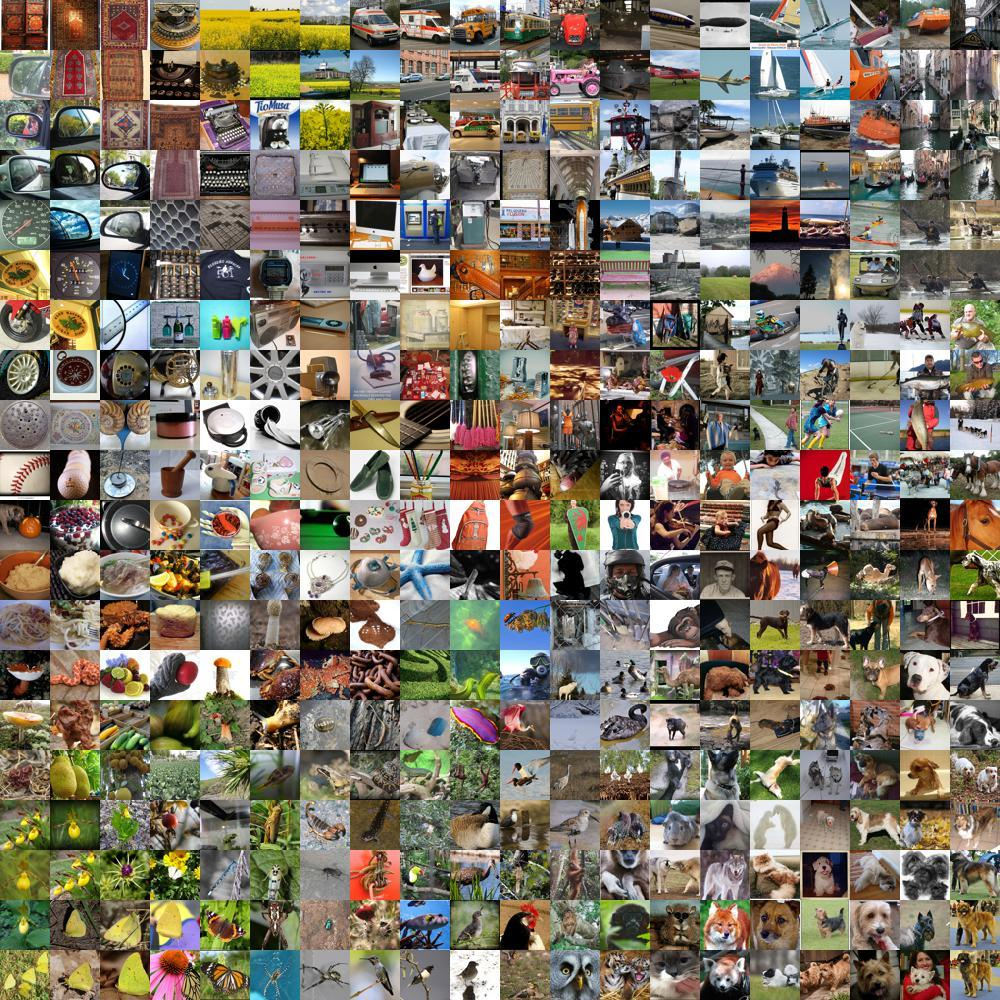
\includegraphics[width=0.8\textwidth]{figures/imagenet}
			\end{figure}

		\end{column}
		
		\begin{column}{.5\textwidth}
			We have three target-tasks $\mathcal{T}_T$ defined by the Rijksmuseum collection

		\end{column}
		
	\end{columns}

\end{frame}

\begin{frame}{On the Transferability of Convolutional Neural Networks}
\end{frame}


\begin{frame}{On the Transferability of Convolutional Neural Networks}
\end{frame}


\begin{frame}{On the Transferability of Convolutional Neural Networks}
\end{frame}


\begin{frame}{On the Transferability of Convolutional Neural Networks}
\end{frame}




\begin{frame}
	\subsection{On the Transferability of Lottery Winners}
\end{frame}


\begin{frame}{On the Transferability of Lottery Winners}

	\begin{center}
		\textcolor{RoyalBlue}{The Lottery Ticket Hypothesis}:
		\textit{"A randomly-initialized dense neural network contains a subnetwork that is initialized such that when trained in isolation it can match the test accuracy of the original network after training for at most the same number of iterations.\footnote{Frankle, Jonathan, and Michael Carbin. "The lottery ticket hypothesis: Finding sparse, trainable neural networks." (2018)}"}
	\end{center}

\end{frame}

\begin{frame}{On the Transferability of Lottery Winners}

	\begin{figure}
		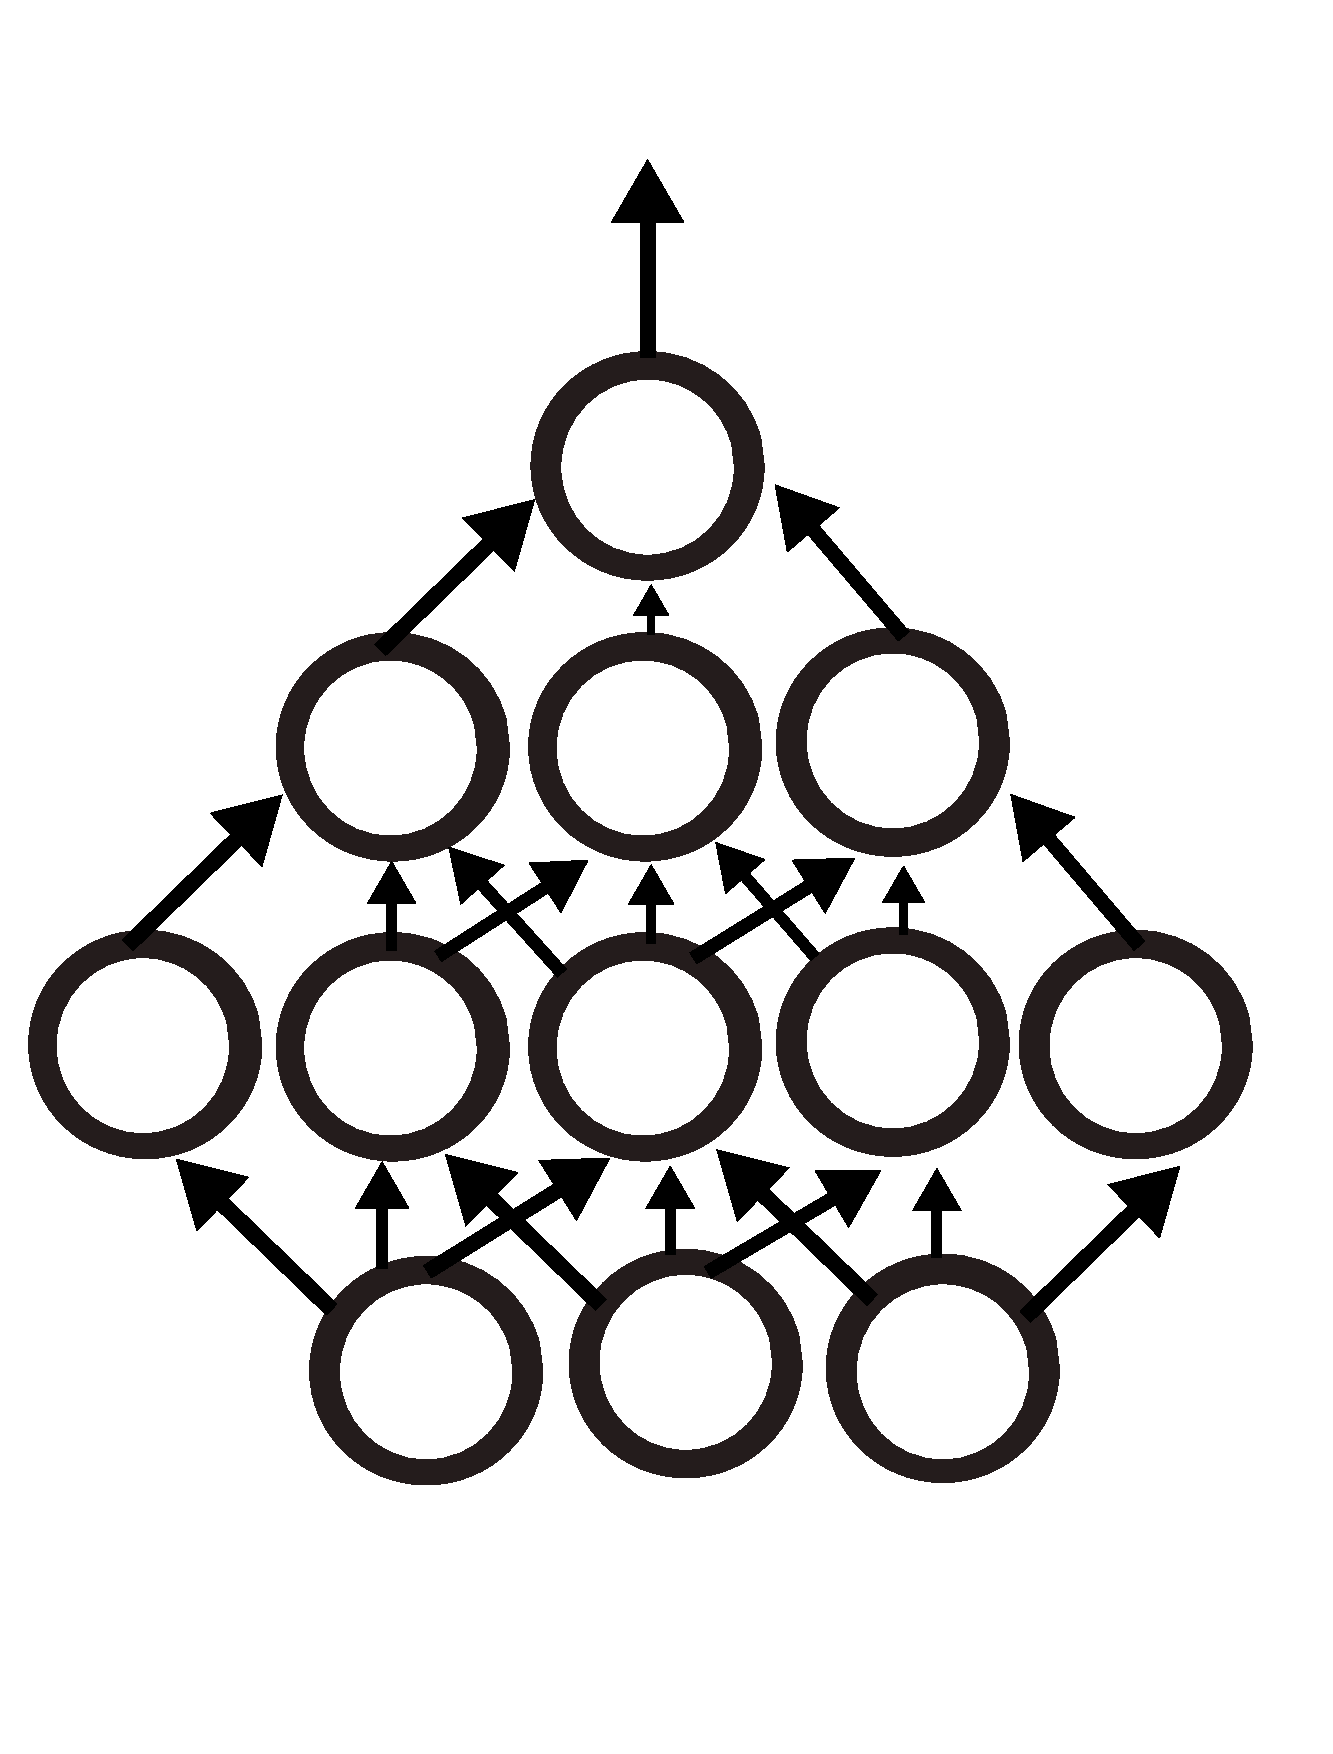
\includegraphics[width=0.5\textwidth]{figures/mlp.pdf}
	\end{figure}

\end{frame}

\begin{frame}{On the Transferability of Lottery Winners}

	\begin{figure}
		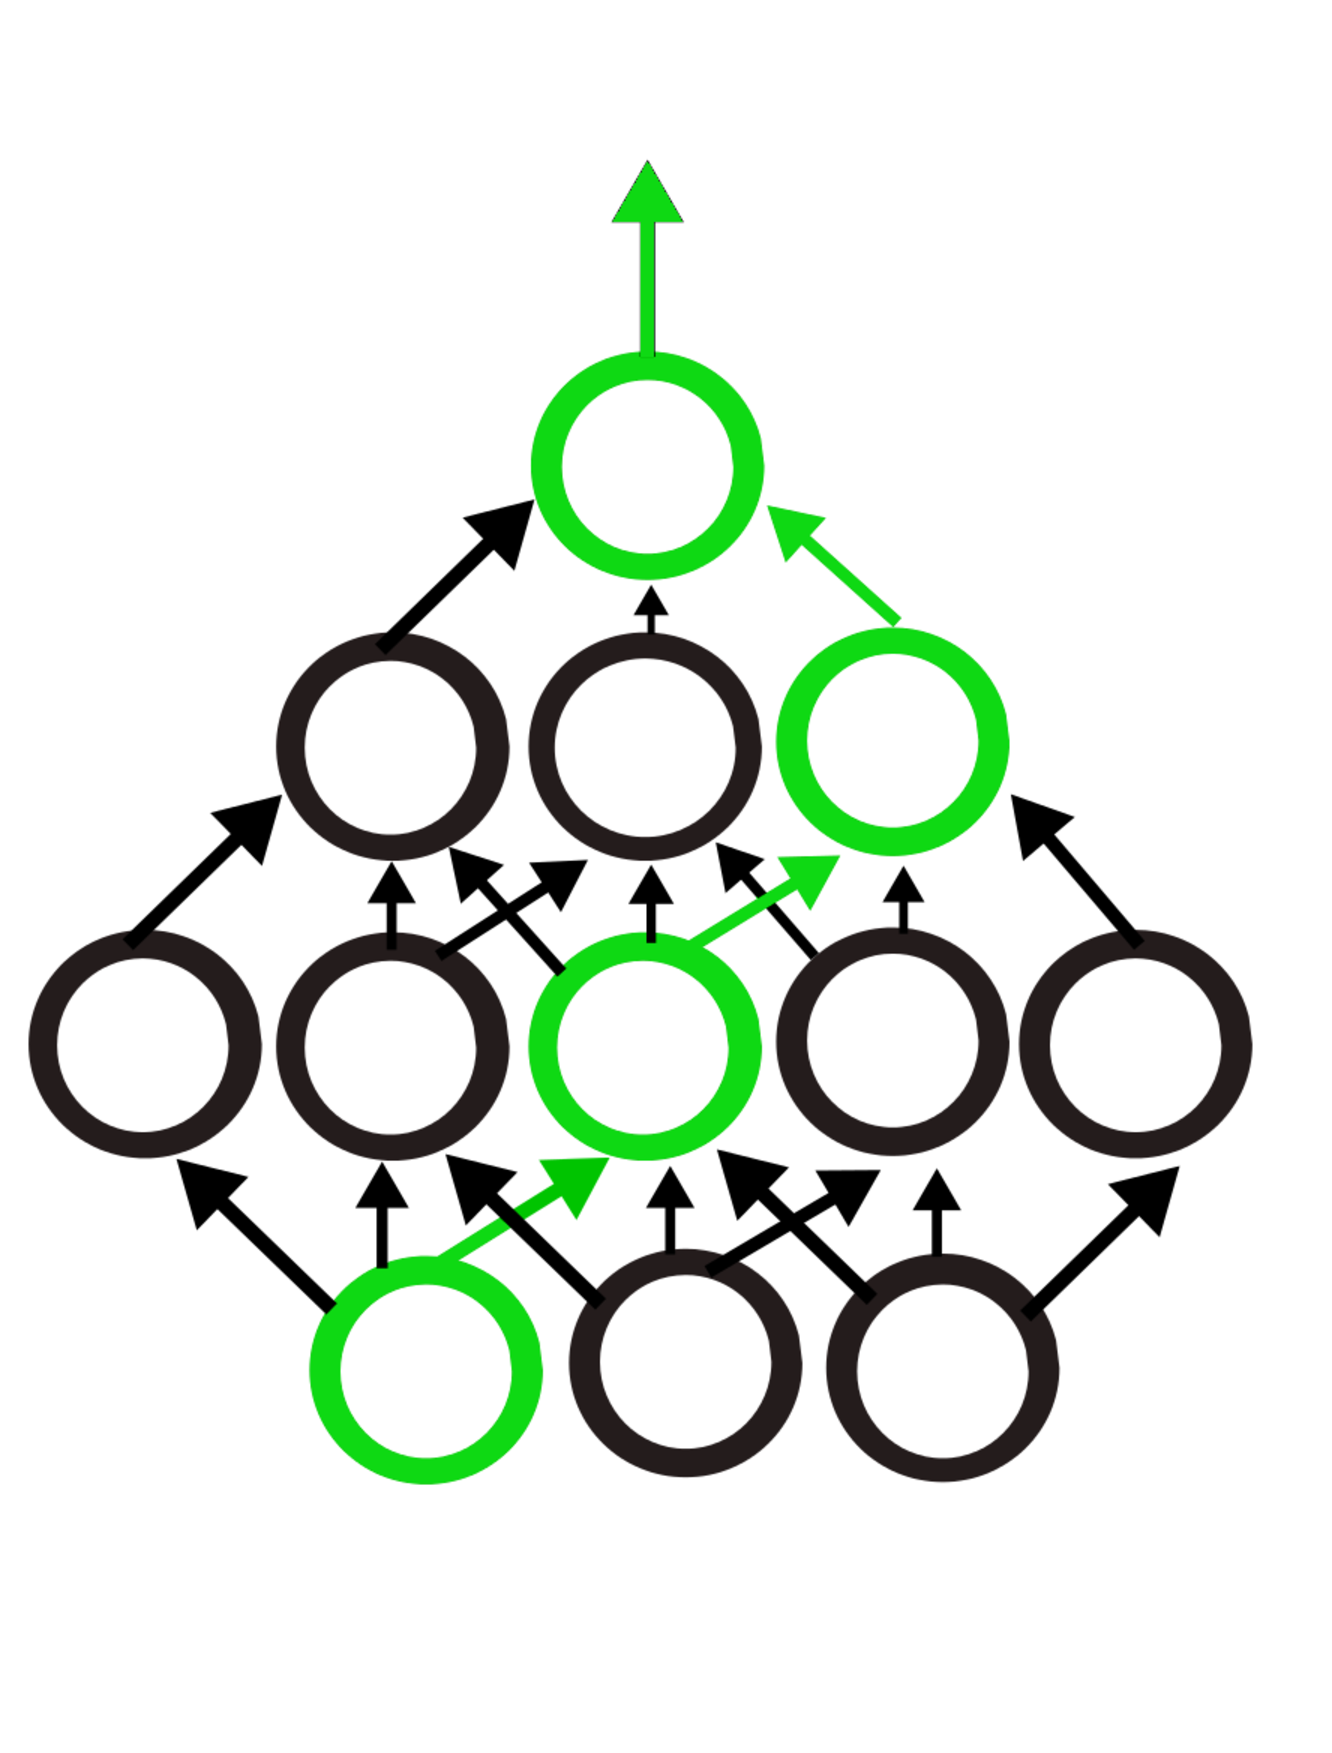
\includegraphics[width=0.5\textwidth]{figures/mlp_ticket_3.pdf}
	\end{figure}

\end{frame}

\begin{frame}{On the Transferability of Lottery Winners}

	\begin{figure}
		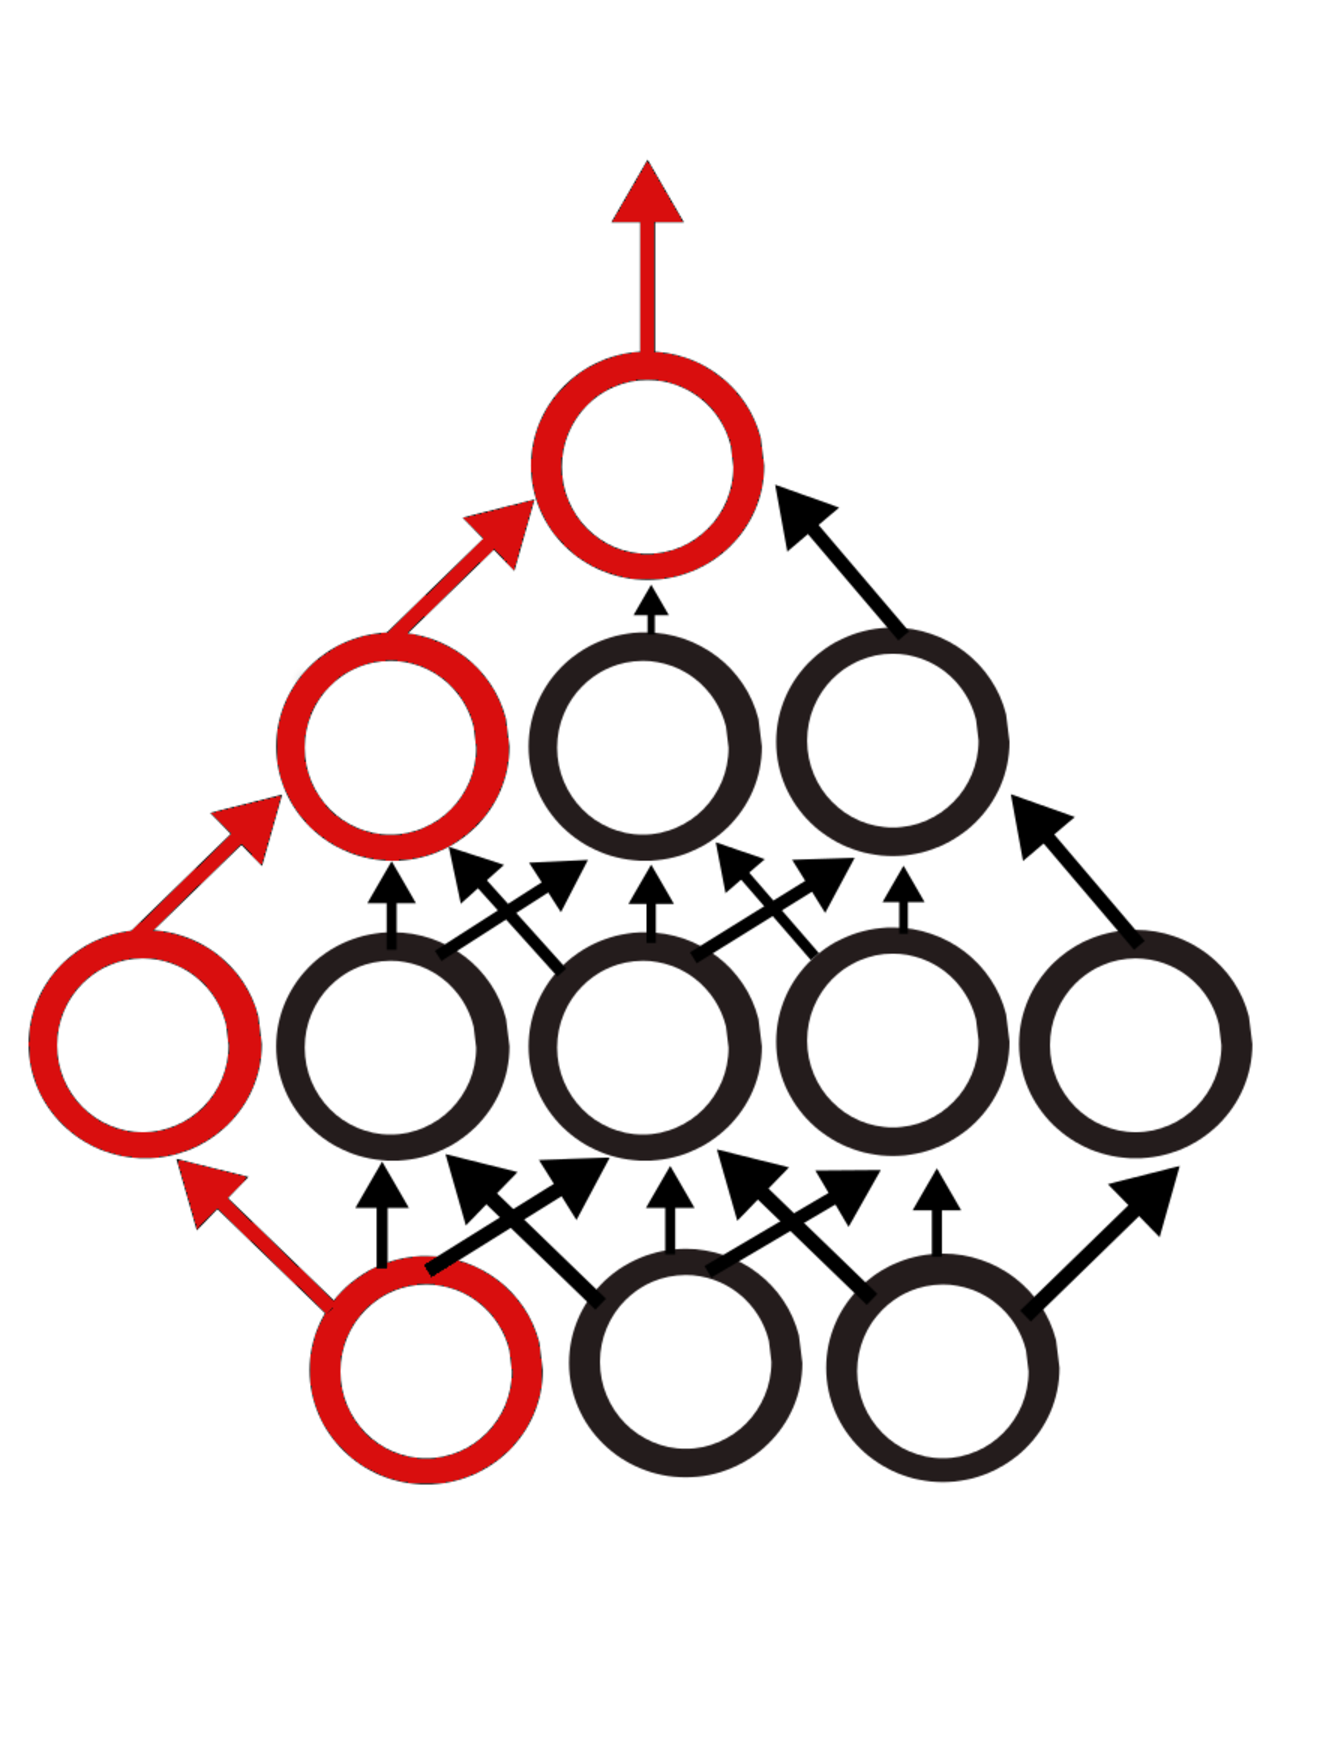
\includegraphics[width=0.5\textwidth]{figures/random_ticket_1.pdf}
	\end{figure}

\end{frame}

\begin{frame}{On the Transferability of Lottery Winners}

	\begin{figure}
		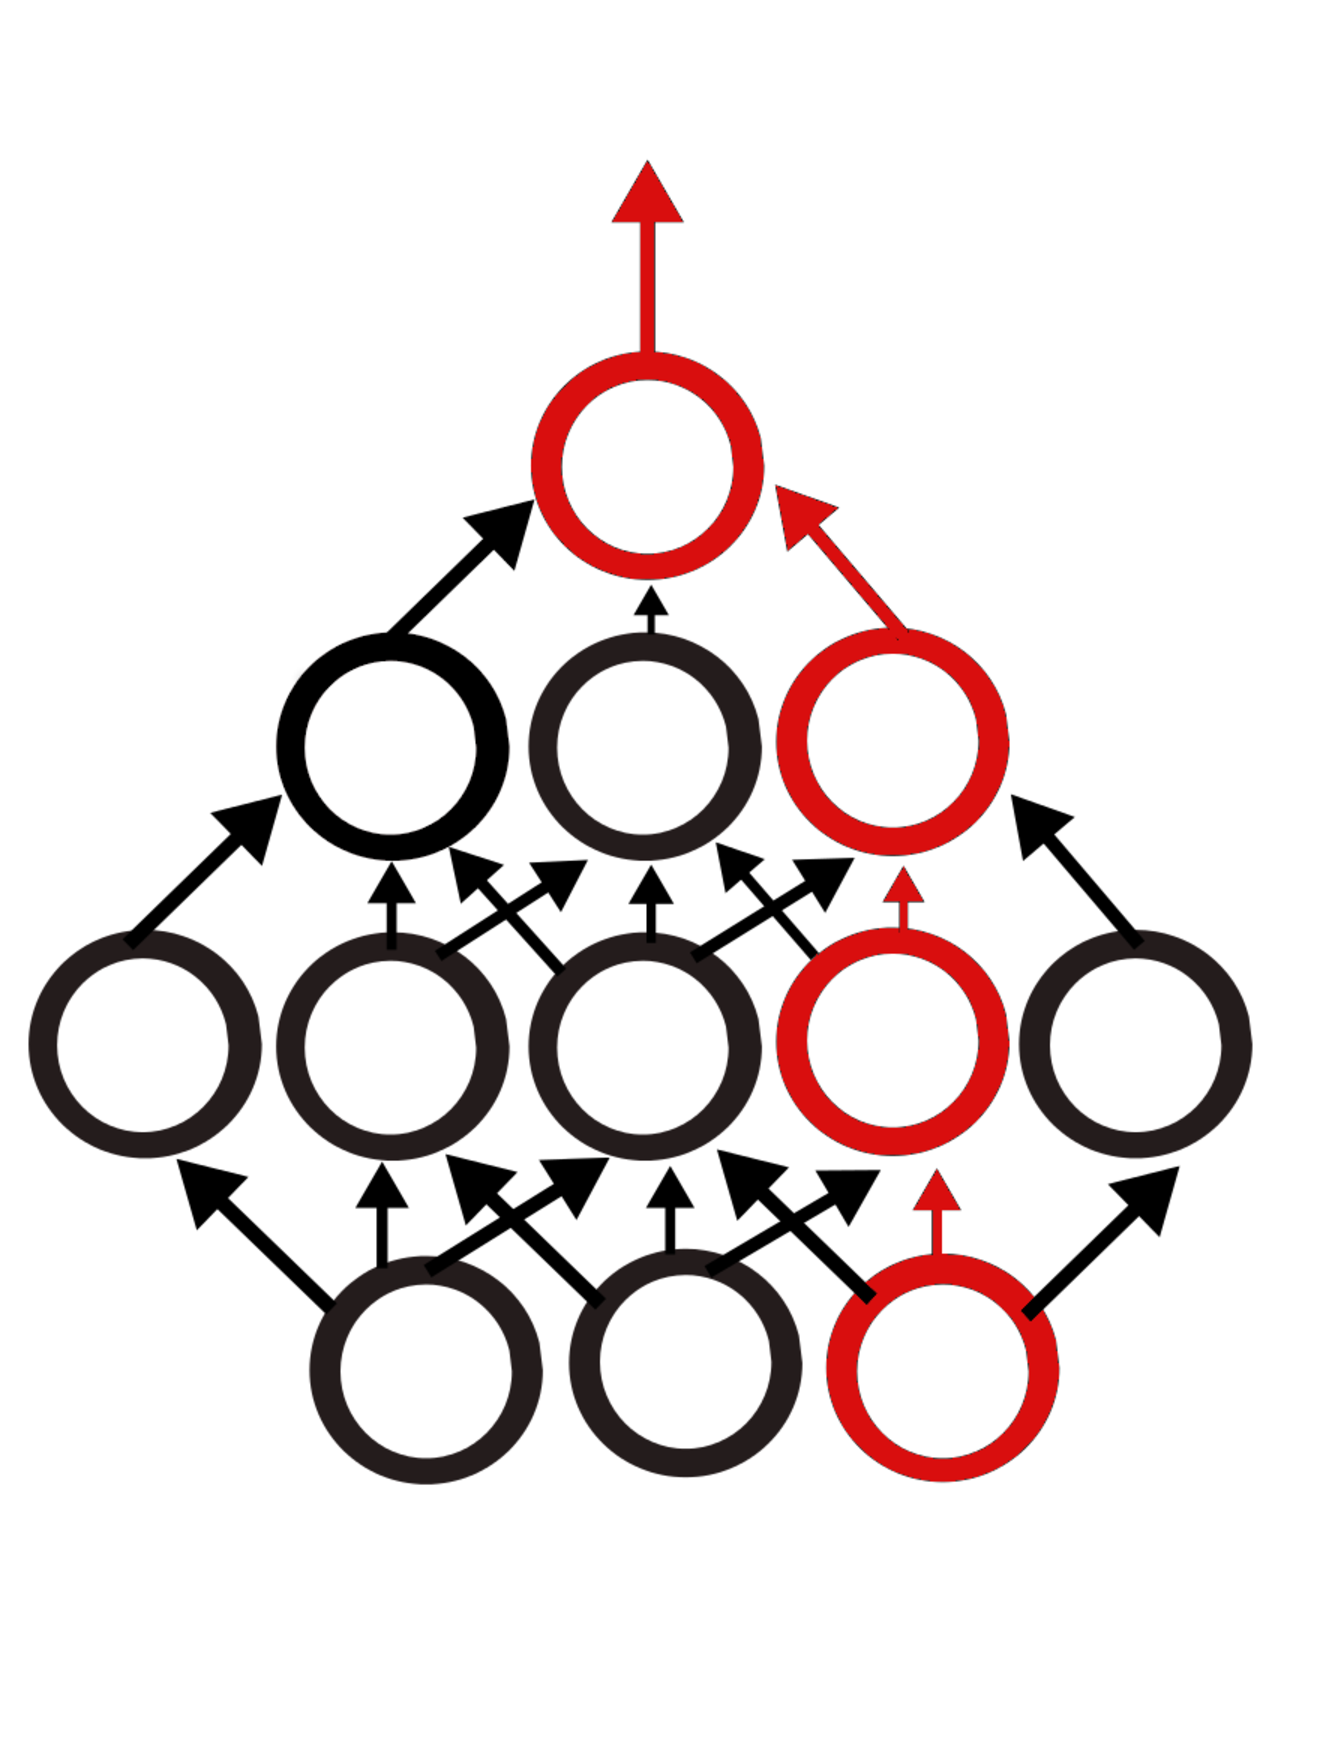
\includegraphics[width=0.5\textwidth]{figures/random_ticket_2.pdf}
	\end{figure}

\end{frame}


\begin{frame}{On the Transferability of Lottery Winners}

	$\Rightarrow$ How does one \textcolor{RoyalBlue}{find} a winning ticket?
	
	\begin{itemize}
		\item Randomly initialize a network $f(x;\theta_0)$ where $\theta_0 \sim \mathcal{D}_{\theta}$
		\item We train the network for $j$ iterations
		\item We prune $p\%$ of the parameters in $\theta_j$ creating a mask $m$
		\item Reset the remaining parameters to their values at $\theta_0$, creating a winning ticket $f(x;m \odot \theta_0)$
	\end{itemize}

\end{frame}


\begin{frame}{On the Transferability of Lottery Winners}
	The Lottery Ticket Hypothesis in practice ...

	\begin{figure}[ht!]
  \centering
  \begin{tikzpicture}[scale = 0.45]
	\begin{axis}[
	grid style={dashed,gray},
	grid = both, 
	tick style=black,
	x label style={at={(axis description cs:0.5,-0.1)},anchor=north},
  	xlabel=Fraction of Weights Pruned,
  	ylabel= Accuracy ($\%$),
	title=CIFAR-10,
	%width=1,
	xtick=data,
	label style={font=\scriptsize},
	xticklabels = {0.0,0.2,0.36,0.488,0.59,0.672,0.738,0.79,0.832,0.866,0.893,0.914,0.931,0.945,0.956,0.965,0.972,0.977,0.982,0.986,0.988,0.991,0.993,0.994,0.995,0.996,0.997,0.998,0.998,0.998,0.999},
	x=4.5mm,
	ymin=0,
    	ymax=90,
	scale only axis,
	xticklabel style={rotate=90},
        %log ticks with fixed point,
        scaled ticks=true,
	/pgf/number format/fixed,
        %log ticks with fixed point,
  	legend pos=outer north east,
]

	\addlegendentry{Baseline}
	\addlegendentry{Winning Ticket $f(x;m\odot\theta_k)$}
	\addlegendentry{Random Mask + Random $\theta$}

\addplot [ultra thick, black, mark=x] table [x expr=\coordindex, y=baseline]{./Chapter06/logs/cifar10_example.txt};
%\addplot [ultra thick, blue, mark=x] table [x expr=\coordindex, y=ticket]{./Chapter06/logs/cifar10_example.txt};
%\addplot [ultra thick, red, mark=x] table [x expr=\coordindex, y=random_mask]{./Chapter06/logs/cifar10_example.txt};

\end{axis}
    \end{tikzpicture}

\end{figure} 

\end{frame}

\begin{frame}{On the Transferability of Lottery Winners}
	The Lottery Ticket Hypothesis in practice ...

	\begin{figure}[ht!]
  \centering
  \begin{tikzpicture}[scale = 0.45]
	\begin{axis}[
	grid style={dashed,gray},
	grid = both, 
	tick style=black,
	x label style={at={(axis description cs:0.5,-0.1)},anchor=north},
  	xlabel=Fraction of Weights Pruned,
  	ylabel= Accuracy ($\%$),
	title=CIFAR-10,
	%width=1,
	xtick=data,
	label style={font=\scriptsize},
	xticklabels = {0.0,0.2,0.36,0.488,0.59,0.672,0.738,0.79,0.832,0.866,0.893,0.914,0.931,0.945,0.956,0.965,0.972,0.977,0.982,0.986,0.988,0.991,0.993,0.994,0.995,0.996,0.997,0.998,0.998,0.998,0.999},
	x=4.5mm,
	ymin=0,
    	ymax=90,
	scale only axis,
	xticklabel style={rotate=90},
        %log ticks with fixed point,
        scaled ticks=true,
	/pgf/number format/fixed,
        %log ticks with fixed point,
  	legend pos=outer north east,
]

	\addlegendentry{Baseline}
	\addlegendentry{Winning Ticket $f(x;m\odot\theta_k)$}
	\addlegendentry{Random Mask + Random $\theta$}

\addplot [ultra thick, black, mark=x] table [x expr=\coordindex, y=baseline]{./Chapter06/logs/cifar10_example.txt};
\addplot [ultra thick, blue, mark=x] table [x expr=\coordindex, y=ticket]{./Chapter06/logs/cifar10_example.txt};
%\addplot [ultra thick, red, mark=x] table [x expr=\coordindex, y=random_mask]{./Chapter06/logs/cifar10_example.txt};

\end{axis}
    \end{tikzpicture}

\end{figure} 

\end{frame}



\begin{frame}{On the Transferability of Lottery Winners}
	The Lottery Ticket Hypothesis in practice ...

	\begin{figure}[ht!]
  \centering
  \begin{tikzpicture}[scale = 0.45]
	\begin{axis}[
	grid style={dashed,gray},
	grid = both, 
	tick style=black,
	x label style={at={(axis description cs:0.5,-0.1)},anchor=north},
  	xlabel=Fraction of Weights Pruned,
  	ylabel= Accuracy ($\%$),
	title=CIFAR-10,
	%width=1,
	xtick=data,
	label style={font=\scriptsize},
	xticklabels = {0.0,0.2,0.36,0.488,0.59,0.672,0.738,0.79,0.832,0.866,0.893,0.914,0.931,0.945,0.956,0.965,0.972,0.977,0.982,0.986,0.988,0.991,0.993,0.994,0.995,0.996,0.997,0.998,0.998,0.998,0.999},
	x=4.5mm,
	ymin=0,
    	ymax=90,
	scale only axis,
	xticklabel style={rotate=90},
        %log ticks with fixed point,
        scaled ticks=true,
	/pgf/number format/fixed,
        %log ticks with fixed point,
  	legend pos=outer north east,
]

	\addlegendentry{Baseline}
	\addlegendentry{Winning Ticket $f(x;m\odot\theta_k)$}
	\addlegendentry{Random Mask + Random $\theta$}

\addplot [ultra thick, black, mark=x] table [x expr=\coordindex, y=baseline]{./Chapter06/logs/cifar10_example.txt};
\addplot [ultra thick, blue, mark=x] table [x expr=\coordindex, y=ticket]{./Chapter06/logs/cifar10_example.txt};
\addplot [ultra thick, red, mark=x] table [x expr=\coordindex, y=random_mask]{./Chapter06/logs/cifar10_example.txt};

\end{axis}
    \end{tikzpicture}

\end{figure} 

\end{frame}

\begin{frame}{On the Transferability of Lottery Winners}
	Why are lottery tickets $f(x;m \odot \theta_0)$ so \textcolor{RoyalBlue}{special}?
	\begin{itemize}
		\item Train faster
		\item Faster Inference
		\item (Sometimes) obtain a better final performance
	\end{itemize}

	However ... 

	\begin{itemize}
		\item Identifying a winning ticket is \textcolor{Maroon}{computationally expensive} 
		\item We \textcolor{Maroon}{do not} know how and why lottery winners appear throughout learning
	\end{itemize}
\end{frame}

\begin{frame}{On the Transferability of Lottery Winners}

	$\Rightarrow$ Therefore we study whether winning tickets $f(x;m \odot \theta_0)$
	found on natural image datasets can get \textcolor{RoyalBlue}{transferred} to the non-natural realm

	\bigskip

	We use three popular Computer Vision datasets as source domains $\mathcal{D}_S$:

	\begin{figure}
 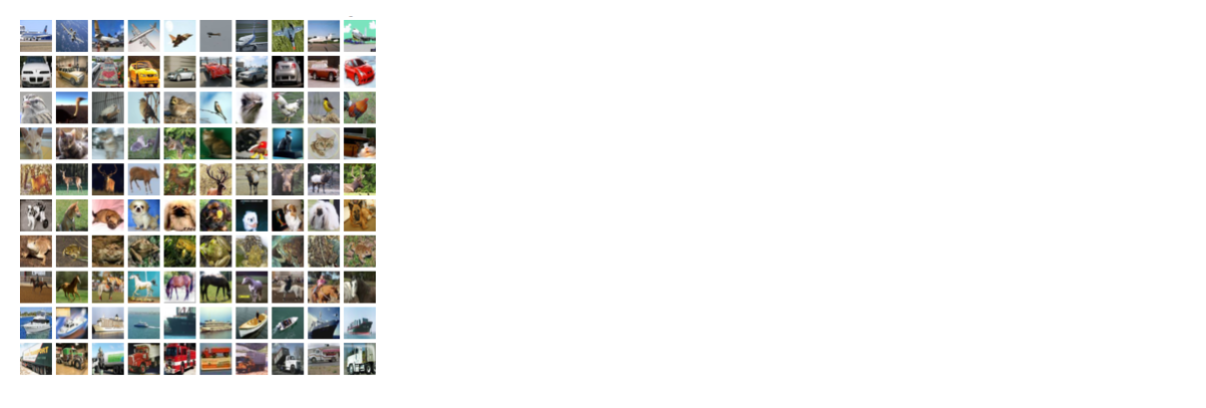
\includegraphics[width=0.8\textwidth]{figures/cifar10}
\end{figure}
\end{frame}

\begin{frame}{On the Transferability of Lottery Winners}

	$\Rightarrow$ Therefore we study whether winning tickets $f(x;m \odot \theta_0)$
	found on natural image datasets can get \textcolor{RoyalBlue}{transferred} to the non-natural realm

	\bigskip

	We use three popular Computer Vision datasets as source domains $\mathcal{D}_S$:

	\begin{figure}
 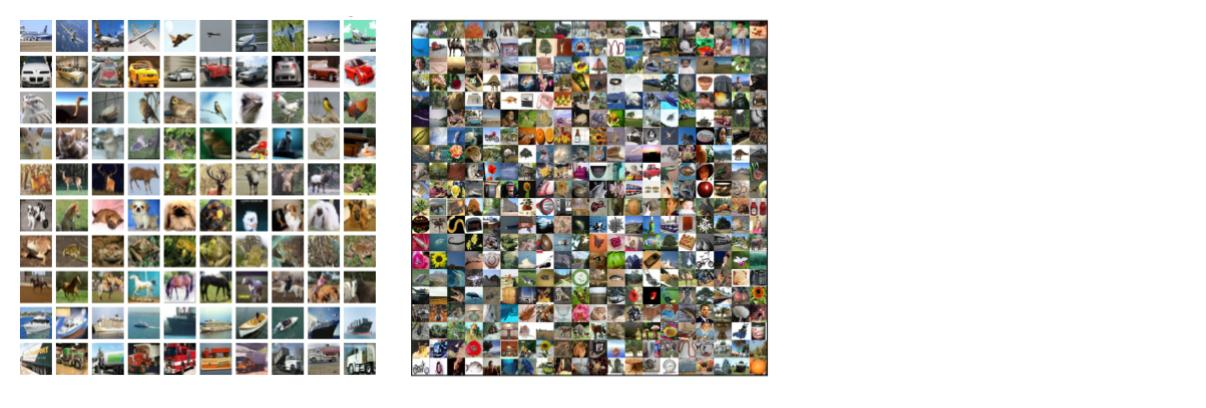
\includegraphics[width=0.8\textwidth]{figures/cifar100}
\end{figure}
\end{frame}

\begin{frame}{On the Transferability of Lottery Winners}

	$\Rightarrow$ Therefore we study whether winning tickets $f(x;m \odot \theta_0)$
	found on natural image datasets can get \textcolor{RoyalBlue}{transferred} to the non-natural realm

	\bigskip

	We use three popular Computer Vision datasets as source tasks $\mathcal{T}_S$

	\begin{figure}
 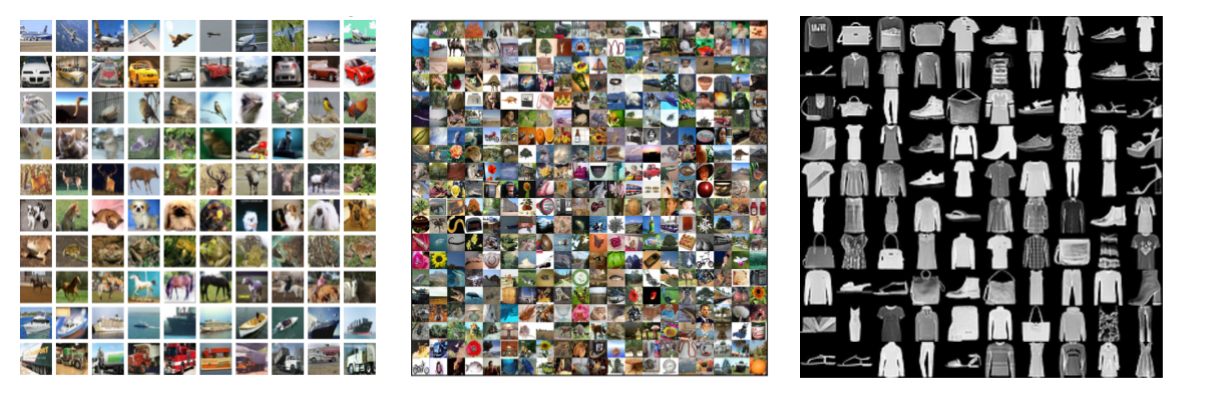
\includegraphics[width=0.8\textwidth]{figures/fashion_mnist}
\end{figure}
\end{frame}


\begin{frame}{On the Transferability of Lottery Winners}

	And we use \textcolor{RoyalBlue}{seven datasets} of non-natural images as target tasks $\mathcal{T}_T$ coming from the fields of Digital Pathology and Digital Heritage

	\begin{figure}
 		\centering
  		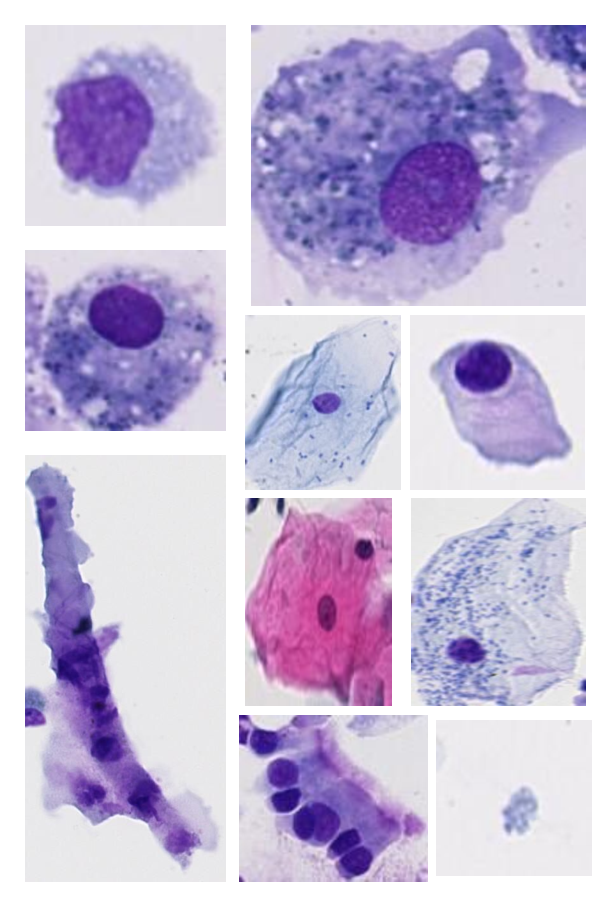
\includegraphics[width=1.8cm,height=\textheight,keepaspectratio]{figures/lba.pdf}%
  		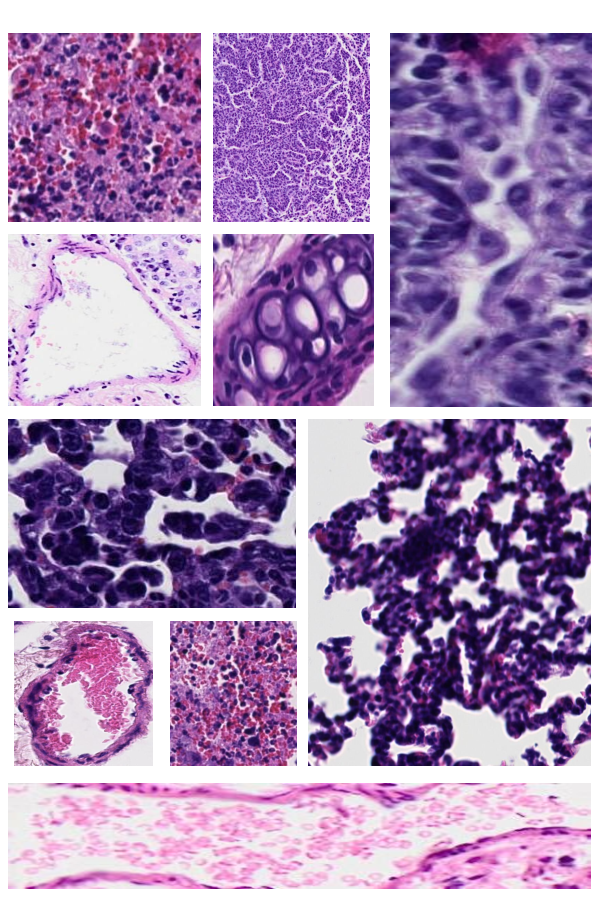
\includegraphics[width=1.8cm,height=\textheight,keepaspectratio]{figures/tissus.pdf}%
  		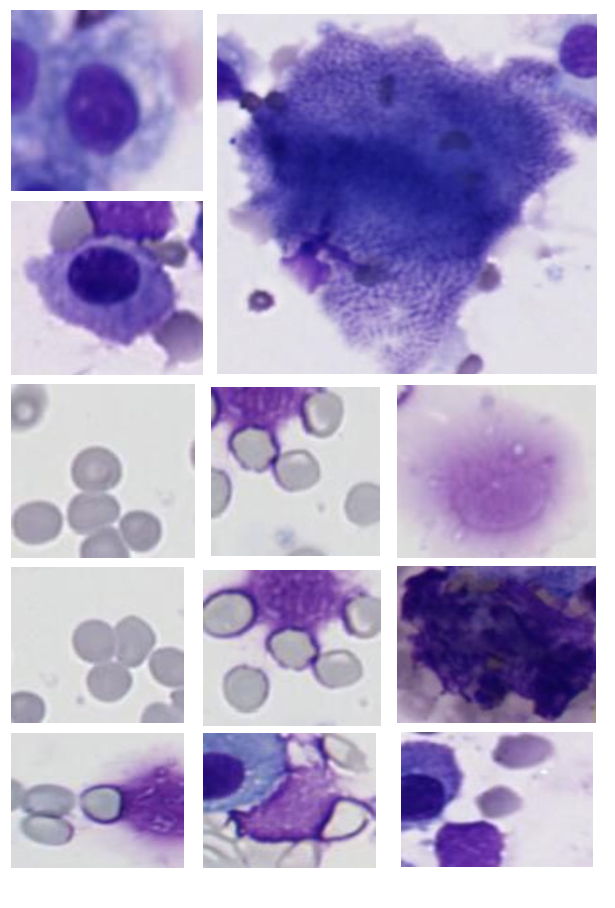
\includegraphics[width=1.8cm,height=\textheight,keepaspectratio]{figures/mouse_lba.pdf}%
  		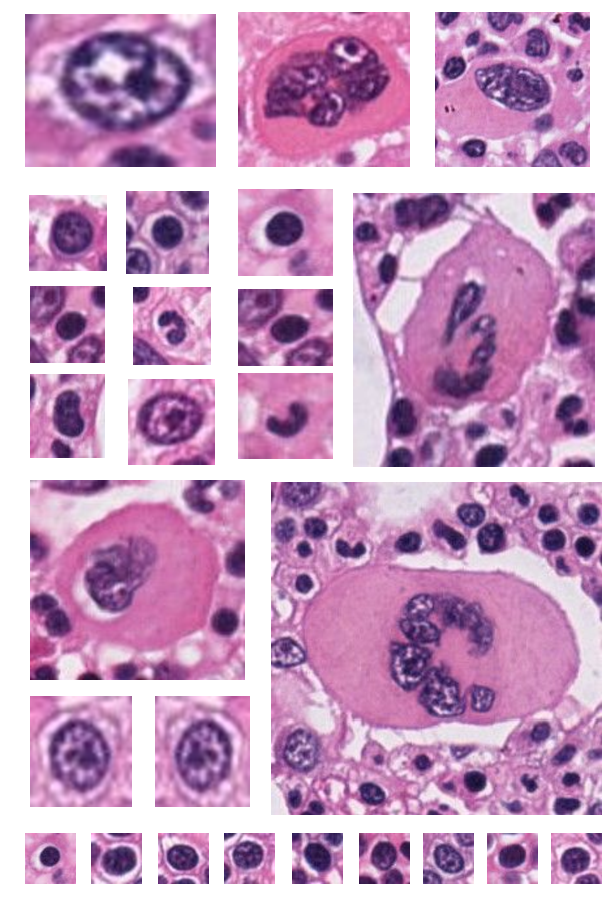
\includegraphics[width=1.8cm,height=\textheight,keepaspectratio]{figures/bonemarrow.pdf}%
    		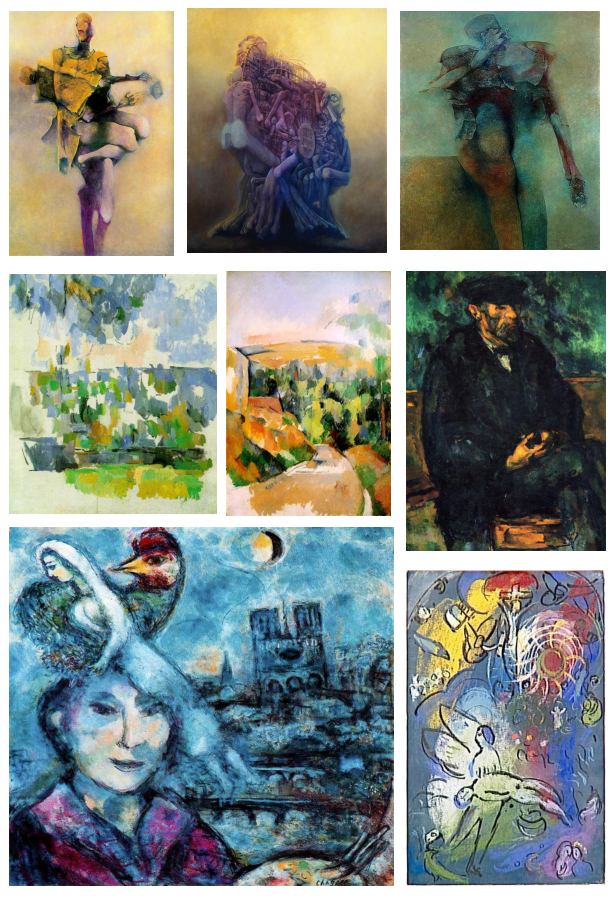
\includegraphics[width=1.8cm,height=\textheight,keepaspectratio]{figures/artist.pdf}%
  		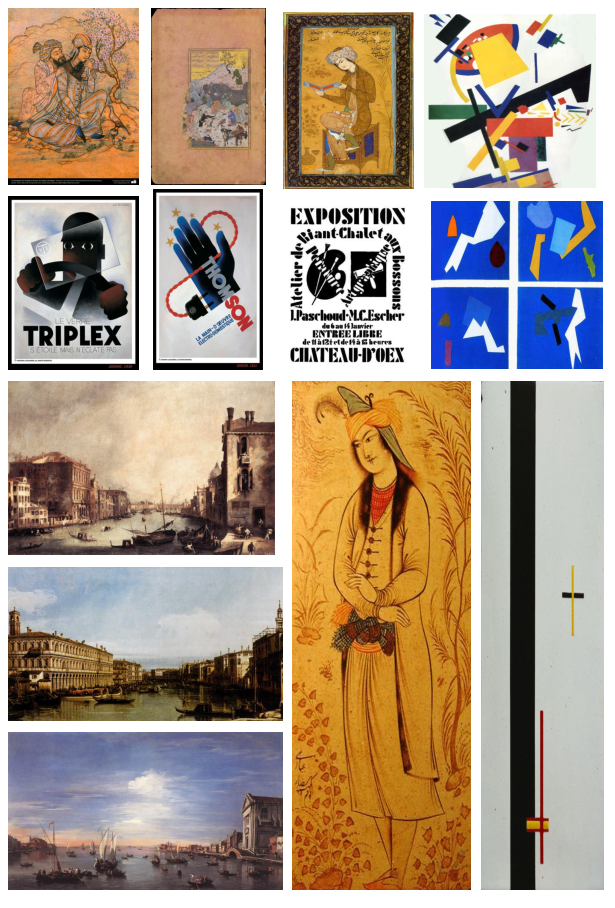
\includegraphics[width=1.8cm,height=\textheight,keepaspectratio]{figures/type.pdf}%
	\end{figure}

\end{frame}


\begin{frame}{On the Transferability of Lottery Winners}
	Transferring lottery winners to the \textcolor{RoyalBlue}{Digital Pathology} data ...
	\begin{figure}[ht!]
\centering
	\begin{tikzpicture}[scale = 0.5]

\begin{axis}[
	name=ax1,
	grid style={dashed,gray},
	grid = both, 
	tick style=black,
  	x label style={at={(axis description cs:0.5,-0.1)},anchor=north},
	xlabel=Fraction of Weights Pruned,
  	ylabel= Accuracy ($\%$),
	ylabel style={font=\Large},
	title=Human-LBA,
	xtick=data,
	legend pos=south west,
	label style={font=\scriptsize},
	xticklabels = {0.0,0.2,0.36,0.488,0.59,0.672,0.738,0.79,0.832,0.866,0.893,0.914,0.931,0.945,0.956,0.965,0.972,0.977,0.982,0.986,0.988,0.991,0.993,0.994,0.995,0.996,0.997,0.998,0.998,0.998,0.999},
	x=4.5mm,
	ymin=40,
    	ymax=90,
	scale only axis,
	xticklabel style={rotate=90},
        %log ticks with fixed point,
        scaled ticks=true,
	/pgf/number format/fixed,
        %log ticks with fixed point,
]

	\addlegendentry{Baseline}
	\addlegendentry{Winning Ticket $f(x;m\odot\theta_k)$}
	\addlegendentry{Random Ticket $f(x;m\odot\theta_r)$}
	\addlegendentry{CIFAR-10}
	\addlegendentry{CIFAR-100}
	\addlegendentry{Fashion-MNIST}


\addplot [ultra thick, black, mark=x] table [x expr=\coordindex, y=baseline]{./Chapter06/logs/human_lba.txt};
%\addplot [ultra thick, blue, mark=x] table [x expr=\coordindex, y=winning_ticket]{./Chapter06/logs/human_lba.txt};
%\addplot [ultra thick, orange, mark=x] table [x expr=\coordindex, y=random_mask]{./Chapter06/logs/human_lba.txt};
%\addplot [ultra thick, green, mark=x] table [x expr=\coordindex, y=cifar10]{./Chapter06/logs/human_lba.txt};
%\addplot [ultra thick, red, mark=x] table [x expr=\coordindex, y=cifar100]{./Chapter06/logs/human_lba.txt};
%\addplot [ultra thick, purple, mark=x] table [x expr=\coordindex, y=fahion_mnist]{./Chapter06/logs/human_lba.txt};

\end{axis}
\end{tikzpicture}
\end{figure} 

\end{frame}

\begin{frame}{On the Transferability of Lottery Winners}
	Transferring lottery winners to the \textcolor{RoyalBlue}{Digital Pathology} data ...
	\begin{figure}[ht!]
\centering
	\begin{tikzpicture}[scale = 0.5]

\begin{axis}[
	name=ax1,
	grid style={dashed,gray},
	grid = both, 
	tick style=black,
  	x label style={at={(axis description cs:0.5,-0.1)},anchor=north},
	xlabel=Fraction of Weights Pruned,
  	ylabel= Accuracy ($\%$),
	ylabel style={font=\Large},
	title=Human-LBA,
	xtick=data,
	legend pos=south west,
	label style={font=\scriptsize},
	xticklabels = {0.0,0.2,0.36,0.488,0.59,0.672,0.738,0.79,0.832,0.866,0.893,0.914,0.931,0.945,0.956,0.965,0.972,0.977,0.982,0.986,0.988,0.991,0.993,0.994,0.995,0.996,0.997,0.998,0.998,0.998,0.999},
	x=4.5mm,
	ymin=40,
    	ymax=90,
	scale only axis,
	xticklabel style={rotate=90},
        %log ticks with fixed point,
        scaled ticks=true,
	/pgf/number format/fixed,
        %log ticks with fixed point,
]

	\addlegendentry{Baseline}
	\addlegendentry{Winning Ticket $f(x;m\odot\theta_k)$}
	\addlegendentry{Random Ticket $f(x;m\odot\theta_r)$}
	\addlegendentry{CIFAR-10}
	\addlegendentry{CIFAR-100}
	\addlegendentry{Fashion-MNIST}


\addplot [ultra thick, black, mark=x] table [x expr=\coordindex, y=baseline]{./Chapter06/logs/human_lba.txt};
\addplot [ultra thick, blue, mark=x] table [x expr=\coordindex, y=winning_ticket]{./Chapter06/logs/human_lba.txt};
%\addplot [ultra thick, orange, mark=x] table [x expr=\coordindex, y=random_mask]{./Chapter06/logs/human_lba.txt};
%\addplot [ultra thick, green, mark=x] table [x expr=\coordindex, y=cifar10]{./Chapter06/logs/human_lba.txt};
%\addplot [ultra thick, red, mark=x] table [x expr=\coordindex, y=cifar100]{./Chapter06/logs/human_lba.txt};
%\addplot [ultra thick, purple, mark=x] table [x expr=\coordindex, y=fahion_mnist]{./Chapter06/logs/human_lba.txt};

\end{axis}
\end{tikzpicture}
\end{figure} 

\end{frame}


\begin{frame}{On the Transferability of Lottery Winners}
		Transferring lottery winners to the \textcolor{RoyalBlue}{Digital Pathology} data ...
\begin{figure}[ht!]
\centering
	\begin{tikzpicture}[scale = 0.5]

\begin{axis}[
	name=ax1,
	grid style={dashed,gray},
	grid = both, 
	tick style=black,
  	x label style={at={(axis description cs:0.5,-0.1)},anchor=north},
	xlabel=Fraction of Weights Pruned,
  	ylabel= Accuracy ($\%$),
	ylabel style={font=\Large},
	title=Human-LBA,
	xtick=data,
	legend pos=south west,
	label style={font=\scriptsize},
	xticklabels = {0.0,0.2,0.36,0.488,0.59,0.672,0.738,0.79,0.832,0.866,0.893,0.914,0.931,0.945,0.956,0.965,0.972,0.977,0.982,0.986,0.988,0.991,0.993,0.994,0.995,0.996,0.997,0.998,0.998,0.998,0.999},
	x=4.5mm,
	ymin=40,
    	ymax=90,
	scale only axis,
	xticklabel style={rotate=90},
        %log ticks with fixed point,
        scaled ticks=true,
	/pgf/number format/fixed,
        %log ticks with fixed point,
]

	\addlegendentry{Baseline}
	\addlegendentry{Winning Ticket $f(x;m\odot\theta_k)$}
	\addlegendentry{Random Ticket $f(x;m\odot\theta_r)$}
	\addlegendentry{CIFAR-10}
	\addlegendentry{CIFAR-100}
	\addlegendentry{Fashion-MNIST}


\addplot [ultra thick, black, mark=x] table [x expr=\coordindex, y=baseline]{./Chapter06/logs/human_lba.txt};
\addplot [ultra thick, blue, mark=x] table [x expr=\coordindex, y=winning_ticket]{./Chapter06/logs/human_lba.txt};
\addplot [ultra thick, orange, mark=x] table [x expr=\coordindex, y=random_mask]{./Chapter06/logs/human_lba.txt};
%\addplot [ultra thick, green, mark=x] table [x expr=\coordindex, y=cifar10]{./Chapter06/logs/human_lba.txt};
%\addplot [ultra thick, red, mark=x] table [x expr=\coordindex, y=cifar100]{./Chapter06/logs/human_lba.txt};
%\addplot [ultra thick, purple, mark=x] table [x expr=\coordindex, y=fahion_mnist]{./Chapter06/logs/human_lba.txt};

\end{axis}
\end{tikzpicture}
\end{figure} 

\end{frame}


\begin{frame}{On the Transferability of Lottery Winners}
		Transferring lottery winners to the \textcolor{RoyalBlue}{Digital Pathology} data ...
\begin{figure}[ht!]
\centering
	\begin{tikzpicture}[scale = 0.5]

\begin{axis}[
	name=ax1,
	grid style={dashed,gray},
	grid = both, 
	tick style=black,
  	x label style={at={(axis description cs:0.5,-0.1)},anchor=north},
	xlabel=Fraction of Weights Pruned,
  	ylabel= Accuracy ($\%$),
	ylabel style={font=\Large},
	title=Human-LBA,
	xtick=data,
	legend pos=south west,
	label style={font=\scriptsize},
	xticklabels = {0.0,0.2,0.36,0.488,0.59,0.672,0.738,0.79,0.832,0.866,0.893,0.914,0.931,0.945,0.956,0.965,0.972,0.977,0.982,0.986,0.988,0.991,0.993,0.994,0.995,0.996,0.997,0.998,0.998,0.998,0.999},
	x=4.5mm,
	ymin=40,
    	ymax=90,
	scale only axis,
	xticklabel style={rotate=90},
        %log ticks with fixed point,
        scaled ticks=true,
	/pgf/number format/fixed,
        %log ticks with fixed point,
]

	\addlegendentry{Baseline}
	\addlegendentry{Winning Ticket $f(x;m\odot\theta_k)$}
	\addlegendentry{Random Ticket $f(x;m\odot\theta_r)$}
	\addlegendentry{CIFAR-10}
	\addlegendentry{CIFAR-100}
	\addlegendentry{Fashion-MNIST}


\addplot [ultra thick, black, mark=x] table [x expr=\coordindex, y=baseline]{./Chapter06/logs/human_lba.txt};
\addplot [ultra thick, blue, mark=x] table [x expr=\coordindex, y=winning_ticket]{./Chapter06/logs/human_lba.txt};
\addplot [ultra thick, orange, mark=x] table [x expr=\coordindex, y=random_mask]{./Chapter06/logs/human_lba.txt};
\addplot [ultra thick, green, mark=x] table [x expr=\coordindex, y=cifar10]{./Chapter06/logs/human_lba.txt};
%\addplot [ultra thick, red, mark=x] table [x expr=\coordindex, y=cifar100]{./Chapter06/logs/human_lba.txt};
%\addplot [ultra thick, purple, mark=x] table [x expr=\coordindex, y=fahion_mnist]{./Chapter06/logs/human_lba.txt};

\end{axis}
\end{tikzpicture}
\end{figure} 

\end{frame}


\begin{frame}{On the Transferability of Lottery Winners}
		Transferring lottery winners to the \textcolor{RoyalBlue}{Digital Pathology} data ...
\begin{figure}[ht!]
\centering
	\begin{tikzpicture}[scale = 0.5]

\begin{axis}[
	name=ax1,
	grid style={dashed,gray},
	grid = both, 
	tick style=black,
  	x label style={at={(axis description cs:0.5,-0.1)},anchor=north},
	xlabel=Fraction of Weights Pruned,
  	ylabel= Accuracy ($\%$),
	ylabel style={font=\Large},
	title=Human-LBA,
	xtick=data,
	legend pos=south west,
	label style={font=\scriptsize},
	xticklabels = {0.0,0.2,0.36,0.488,0.59,0.672,0.738,0.79,0.832,0.866,0.893,0.914,0.931,0.945,0.956,0.965,0.972,0.977,0.982,0.986,0.988,0.991,0.993,0.994,0.995,0.996,0.997,0.998,0.998,0.998,0.999},
	x=4.5mm,
	ymin=40,
    	ymax=90,
	scale only axis,
	xticklabel style={rotate=90},
        %log ticks with fixed point,
        scaled ticks=true,
	/pgf/number format/fixed,
        %log ticks with fixed point,
]

	\addlegendentry{Baseline}
	\addlegendentry{Winning Ticket $f(x;m\odot\theta_k)$}
	\addlegendentry{Random Ticket $f(x;m\odot\theta_r)$}
	\addlegendentry{CIFAR-10}
	\addlegendentry{CIFAR-100}
	\addlegendentry{Fashion-MNIST}


\addplot [ultra thick, black, mark=x] table [x expr=\coordindex, y=baseline]{./Chapter06/logs/human_lba.txt};
\addplot [ultra thick, blue, mark=x] table [x expr=\coordindex, y=winning_ticket]{./Chapter06/logs/human_lba.txt};
\addplot [ultra thick, orange, mark=x] table [x expr=\coordindex, y=random_mask]{./Chapter06/logs/human_lba.txt};
\addplot [ultra thick, green, mark=x] table [x expr=\coordindex, y=cifar10]{./Chapter06/logs/human_lba.txt};
\addplot [ultra thick, red, mark=x] table [x expr=\coordindex, y=cifar100]{./Chapter06/logs/human_lba.txt};
%\addplot [ultra thick, purple, mark=x] table [x expr=\coordindex, y=fahion_mnist]{./Chapter06/logs/human_lba.txt};

\end{axis}
\end{tikzpicture}
\end{figure} 

\end{frame}

\begin{frame}{On the Transferability of Lottery Winners}
	Transferring lottery winners to the \textcolor{RoyalBlue}{Digital Pathology} data ...
	\begin{figure}[ht!]
\centering
	\begin{tikzpicture}[scale = 0.5]

\begin{axis}[
	name=ax1,
	grid style={dashed,gray},
	grid = both, 
	tick style=black,
  	x label style={at={(axis description cs:0.5,-0.1)},anchor=north},
	xlabel=Fraction of Weights Pruned,
  	ylabel= Accuracy ($\%$),
	ylabel style={font=\Large},
	title=Human-LBA,
	xtick=data,
	legend pos=south west,
	label style={font=\scriptsize},
	xticklabels = {0.0,0.2,0.36,0.488,0.59,0.672,0.738,0.79,0.832,0.866,0.893,0.914,0.931,0.945,0.956,0.965,0.972,0.977,0.982,0.986,0.988,0.991,0.993,0.994,0.995,0.996,0.997,0.998,0.998,0.998,0.999},
	x=4.5mm,
	ymin=40,
    	ymax=90,
	scale only axis,
	xticklabel style={rotate=90},
        %log ticks with fixed point,
        scaled ticks=true,
	/pgf/number format/fixed,
        %log ticks with fixed point,
]

	\addlegendentry{Baseline}
	\addlegendentry{Winning Ticket $f(x;m\odot\theta_k)$}
	\addlegendentry{Random Ticket $f(x;m\odot\theta_r)$}
	\addlegendentry{CIFAR-10}
	\addlegendentry{CIFAR-100}
	\addlegendentry{Fashion-MNIST}


\addplot [ultra thick, black, mark=x] table [x expr=\coordindex, y=baseline]{./Chapter06/logs/human_lba.txt};
\addplot [ultra thick, blue, mark=x] table [x expr=\coordindex, y=winning_ticket]{./Chapter06/logs/human_lba.txt};
\addplot [ultra thick, orange, mark=x] table [x expr=\coordindex, y=random_mask]{./Chapter06/logs/human_lba.txt};
\addplot [ultra thick, green, mark=x] table [x expr=\coordindex, y=cifar10]{./Chapter06/logs/human_lba.txt};
\addplot [ultra thick, red, mark=x] table [x expr=\coordindex, y=cifar100]{./Chapter06/logs/human_lba.txt};
\addplot [ultra thick, purple, mark=x] table [x expr=\coordindex, y=fahion_mnist]{./Chapter06/logs/human_lba.txt};

\end{axis}
\end{tikzpicture}
\end{figure} 

\end{frame}

\begin{frame}{On the Transferability of Lottery Winners}
	Transferring lottery winners to the \textcolor{RoyalBlue}{Digital Heritage} data ...
	\begin{figure}[ht!]
\centering
	\begin{tikzpicture}[scale = 0.5]
\begin{axis}[
	name=ax1,
	grid style={dashed,gray},
	grid = both, 
	tick style=black,
	x label style={at={(axis description cs:0.5,-0.1)},anchor=north},
  	xlabel=Fraction of Weights Pruned,
  	ylabel= Accuracy ($\%$),
	title=Artist Classification 1,
	%width=1,
	xtick=data,
	legend pos=south west,
	label style={font=\scriptsize},
	xticklabels = {0.0,0.2,0.36,0.488,0.59,0.672,0.738,0.79,0.832,0.866,0.893,0.914,0.931,0.945,0.956,0.965,0.972,0.977,0.982,0.986,0.988,0.991,0.993,0.994,0.995,0.996,0.997,0.998,0.998,0.998,0.999},
	x=4.5mm,
	ymin=0,
    	ymax=75,
	scale only axis,
	xticklabel style={rotate=90},
        %log ticks with fixed point,
        scaled ticks=true,
	/pgf/number format/fixed,
        %log ticks with fixed point,
  	%legend pos=outer north east,
	%legend style={font=\small, at={(-0.8,-0.2,-0.2)},anchor=north west, legend columns = 1}
	]

	\addlegendentry{Baseline}
	\addlegendentry{Winning Ticket $f(x;m\odot\theta_k)$}
	\addlegendentry{Random Ticket $f(x;m\odot\theta_r)$}
	\addlegendentry{CIFAR-10}
	\addlegendentry{CIFAR-100}
	\addlegendentry{Fashion-MNIST}


\addplot [ultra thick, black, mark=x] table [x expr=\coordindex, y=baseline]{./Chapter06/logs/artist_classification_1.txt};
\addplot [ultra thick, blue, mark=x] table [x expr=\coordindex, y=winning_ticket]{./Chapter06/logs/artist_classification_1.txt};
\addplot [ultra thick, orange, mark=x] table [x expr=\coordindex, y=random_mask]{./Chapter06/logs/artist_classification_1.txt};
\addplot [ultra thick, green, mark=x] table [x expr=\coordindex, y=cifar10]{./Chapter06/logs/artist_classification_1.txt};
\addplot [ultra thick, red, mark=x] table [x expr=\coordindex, y=cifar100]{./Chapter06/logs/artist_classification_1.txt};
\addplot [ultra thick, purple, mark=x] table [x expr=\coordindex, y=fahion_mnist]{./Chapter06/logs/artist_classification_1.txt};

\end{axis}    
\end{tikzpicture}
\end{figure} 

\end{frame}



\begin{frame}{On the Transferability of Lottery Winners}

	Our main findings show that on Digital Pathology data
	\bigskip
	\begin{itemize}
		\item All lottery winners \textcolor{RoyalBlue}{significantly outperfom} unpruned models 
		\item Natural lottery winners contain \textcolor{RoyalBlue}{a generic inductive bias} (to some extent)
		\item Best performance is obtained by identifying a winning ticket directly on the \textcolor{Maroon}{target task} $\mathcal{T}_T$
	\end{itemize}
	\bigskip

	whereas on Digital Heritage data
	\bigskip
	\begin{itemize}
		\item Natural lottery winners transfer \textcolor{RoyalBlue}{much better}
		\item They can even \textcolor{RoyalBlue}{outperform} target task $\mathcal{T}_T$ tickets
	\end{itemize}
\end{frame}

\begin{frame}{On the Transferability of Lottery Winners}
	
	We also provide additional empirical insights into the Lottery Ticket Hypothesis:

	\begin{itemize}
		\item We show that completely pre-trained winning tickets $f(x;m \odot \theta_i)$ \textcolor{Maroon}{overfit} on the source task $\mathcal{T}_S$ 
		\item The presence of winning tickets \textcolor{Maroon}{does not depend} on the size of the training data
		\item The closer the source task $\mathcal{S}_T$ and the target task $\mathcal{T}_T$ the \textcolor{RoyalBlue}{better} the transferability of $f(x;m \odot \theta_k)$
	\end{itemize}

\end{frame}

%============================================================================

\begin{frame}
	\begin{center}
		\textcolor{skymagenta}{\textbf{PART III}}
	\end{center}
\end{frame}


%============================================================================


\begin{frame}{A Novel Family of Deep Reinforcement Learning Algorithms}
	\section{Part III: Reinforcement Learning}
	\subsection{A Novel Family of Deep Reinforcement Learning Algorithms}

	\bigskip
	We now consider a different machine learning paradigm: \textcolor{RoyalBlue}{Reinforcement Learning} (RL), where an agent needs to learn how to interact with its environment

	\begin{figure}[htb!]
		\centering
		\tikzset{
  frame/.style={
    rectangle, draw,
    text width=6em, text centered,
    minimum height=4em,drop shadow,fill=white,
    rounded corners,
  },
  line/.style={
    draw, -{Latex},rounded corners=3mm,
  }
}

\begin{tikzpicture}[font=\small\sffamily\bfseries,very thick,node distance = 4cm]
\node [frame] (agent) {Agent};
\node [frame, below=1.2cm of agent] (environment) {Environment};
\draw[line] (agent.0) -- ++ (1.5,0) |- (environment.0) 
node[right,pos=0.25,align=left] {action\\ $a_t$};
\coordinate[left=8mm of environment] (P);
\draw[thin,dashed] (P|-environment.north) -- (P|-environment.south);
\draw[line] (environment.200) -- (P |- environment.200)
node[midway,above]{$s_{t+1}$};
\draw[line,thick] (environment.160) -- (P |- environment.160)
node[midway,above]{$r_{t+1}$};
\draw[line] (P |- environment.200) -- ++ (-1.4,0) |- (agent.160)
node[left, pos=0.25, align=right] {state\\ $s_t$};
\draw[line,thick] (P |- environment.160) -- ++ (-0.8,0) |- (agent.200)
node[right,pos=0.25,align=left] {reward\\ $r_t$};
\end{tikzpicture}


 		\label{fig:rl_loop}
	\end{figure}

\end{frame}

\begin{frame}{A Novel Family of Deep Reinforcement Learning Algorithms}

	Such interaction is modeled as a \textcolor{RoyalBlue}{Markov Decision Process} (MDP) consisting of the following elements:

\begin{itemize}
	\item A set of possible states $\mathcal{S}$,
	\item A set of possible actions $\mathcal{A}$,
	\item A transition function $\mathcal{P}:\mathcal{S}\times\mathcal{A}\times\mathcal{S}\rightarrow [0,1]$,
	\item A reward function $\Re:\mathcal{S}\times\mathcal{A}\times\mathcal{S}\rightarrow \mathbb{R}$,
	\item A discount factor denoted as $\gamma \in [0,1]$.
\end{itemize}

\bigskip

Therefore we can define an MDP as $\mathcal{M}=\langle\mathcal{S}, \mathcal{A}, \mathcal{P}, \Re, \gamma\rangle$.

\end{frame}

\begin{frame}{A Novel Family of Deep Reinforcement Learning Algorithms}
	
	\bigskip

	The interaction between the agent and the environment is given by the agent's \textcolor{RoyalBlue}{policy} $\pi$, a probability distribution over $a \in \mathcal{A}(s)$ for each $s \in \mathcal{S}$:

	\begin{equation*}
	\pi(a|s) = \text{Pr}\; \{a_t = a | s_t = s\}, \; \text{for all}\; s \in \mathcal{S}\; \text{and}\; a\ \in \mathcal{A}.
	\end{equation*}

	\bigskip

	The \textcolor{RoyalBlue}{goal} of the agent is to maximize the expected discounted return as:
	\begin{equation*}
		\begin{split}
			G_t & = r_t+\gamma r_{t+1} + \gamma^{2} r_{t+2} + ... \\
	    			& = \sum_{k=0}^{\infty}\gamma^{k} r_{t+k}.
		\end{split}
		\label{eq:discounted_return}
	\end{equation*}

\end{frame}


\begin{frame}{A Novel Family of Deep Reinforcement Learning Algorithms}
	
	\bigskip
	In RL some components of the MDP are unknown 
	\begin{center}
		$\mathcal{M}=\langle\mathcal{S}, \mathcal{A}, \textcolor{red}{\mathcal{P}}, \textcolor{red}{\Re}, \gamma\rangle$,
	\end{center}
	
	which in the case of \textcolor{RoyalBlue}{model-free} RL can be overcome by learning either the state-value function

	\begin{align*}
    		V^{\pi}(s)=\mathds{E}\bigg[\sum_{k=0}^{\infty}\gamma^{k}r_{t+k}\bigg| s_t = s, \pi \bigg],
	\end{align*}

	or the state-action value function

	\begin{align*}
     		Q^{\pi}(s,a)=\mathds{E}\bigg[\sum_{k=0}^{\infty}\gamma^{k}r_{t+k} \bigg| s_t = s, a_t=a, \pi\bigg].
	\end{align*}
\end{frame}


\begin{frame}{A Novel Family of Deep Reinforcement Learning Algorithms}
	\begin{itemize}
		\item Model-free algorithms are implemented in a \textcolor{RoyalBlue}{tabular} fashion, meaning that the state values, or state-action values, are stored within tables of sizes $|\mathcal{S}|$ and $|\mathcal{S}\times\mathcal{A}|$ respectively

		\item For many problems we typically seek to learn an \textcolor{RoyalBlue}{approximation} of the value functions
	\end{itemize}
	
	\begin{center}

		$V^{\pi}(s)\approx V^\pi{(s;\theta)}$ and $Q^{\pi}(s,a;\theta)\approx Q(s,a;\theta)$
	\end{center}

\end{frame}


\begin{frame}{A Novel Family of Deep Reinforcement Learning Algorithms}

	This approximation can be represented by a \textcolor{RoyalBlue}{Convolutional Neural Network}

\end{frame}


\begin{frame}{A Novel Family of Deep Reinforcement Learning Algorithms}

	Typical DRL algorithms aim at only learning an approximation of the state-action value function $Q^{\pi}(s,a)\approx Q^{\pi}(s,a;\theta)$

	\begin{itemize}
		\item A policy $\pi$ can only be derived from $Q^{\pi}(s,a)$ 
		\item It is hard to combine RL algorithms with neural networks
		\item Dealing with one value function is enough
	\end{itemize}

	\bigskip

	However ...

	\begin{itemize}
		\item Training can be very slow 
		\item Algorithms are prone to diverge
		\item Do not correctly estimate $Q^{\pi}(s,a)$
	\end{itemize}

\end{frame}

\begin{frame}{A Novel Family of Deep Reinforcement Learning Algorithms}
	\bigskip

	$\Rightarrow$ Therefore we suggest to \textcolor{RoyalBlue}{jointly approximate} the state-value function $V^{\pi}(s;\phi)$ alongside the state-action value function $Q^{\pi}(s,a;\theta)$

	\bigskip

	We can do this by either learning $V^{\pi}(s;\phi)$ with
		\begin{multline*}
L(\phi) = \mathds{E}_{\langle s_{t},a_{t},r_{t},s_{t+1}\rangle\sim U(D)} \bigg[\big(r_{t} + \gamma V(s_{t+1}; \Phi^{-}) - V(s_{t}; \Phi)\big)^{2}\bigg],
		\end{multline*}			
		and $Q^{\pi}(s,a)$ with:
		\begin{multline*}
    			L(\theta) = \mathds{E}_{\langle s_{t},a_{t},r_{t},s_{t+1}\rangle\sim U(D)} \bigg[\big(r_{t} + \gamma V(s_{t+1}; \Phi^{-}) - Q(s_{t}, a_{t}; \theta)\big)^{2}\bigg],
		\end{multline*}

\end{frame}

\begin{frame}{A Novel Family of Deep Reinforcement Learning Algorithms}

	... or by learning $V^{\pi}(s;\phi)$ with
	\begin{multline*}
		L(\phi) = \mathds{E}_{\langle s_{t},a_{t},r_{t},s_{t+1}\rangle\sim U(D)} \bigg[\big(r_{t} + \gamma \: \underset{a\in \mathcal{A}}{\max}\: Q(s_{t+1}, a; \theta^{-}) - V(s_{t}; \Phi)\big)^{2}\bigg],
	\end{multline*}
	and $Q^{\pi}(s,a)$ with:
	\begin{multline*}
    		L(\theta) = \mathds{E}_{\langle s_{t},a_{t},r_{t},s_{t+1}\rangle\sim U(D)} \bigg[\big(r_{t} + \gamma V(s_{t+1}; \Phi) - Q(s_{t}, a_{t}; \theta)\big)^{2}\bigg].
	\end{multline*}
\end{frame}

\begin{frame}{A Novel Family of Deep Reinforcement Learning Algorithms}
	The first two objective functions constitute the \textcolor{skymagenta}{\textbf{DQV-Learning}} algorithm, whereas the second two objective functions define the \textcolor{skymagenta}{\textbf{DQV-Max Learning}} algorithm.


	\bigskip

	We compare their performance to algorithms which only learn an approximation of the state-action value function $Q^\pi(s,a)$

\end{frame}

\begin{frame}{A Novel Family of Deep Reinforcement Learning Algorithms}
	\begin{figure}[ht!]
  \begin{tikzpicture}[scale = 0.4]
      \begin{axis}[
	name=ax1,
      	grid style={dashed,gray},
      	grid = both, 
      	tick style=black,
	title=Boxing,
        xlabel=Episodes,
        ylabel=Reward,
      ]


      %\addlegendentry{DQV} 
      %\addlegendentry{DQV-Max}  
      \addlegendentry{DQN}
      \addlegendentry{DDQN}
      
      %\addplot [ultra thick, red, mark=.] table [y=DQV, x=episodes]
      %{./Chapter07/logs/boxing_results.txt};
      % \addplot [ultra thick, yellow, mark=.] table [y=DQV-Max, x=episodes]
      %{./Chapter07/logs/boxing_results.txt};
      \addplot [ultra thick, blue, mark=.] table [y=DQN, x=episodes]{./Chapter07/logs/boxing_results.txt};
      \addplot [ultra thick, green, mark=.] table [y=DDQN, x=episodes]{./Chapter07/logs/boxing_results.txt};
     
      \legend{}

      \end{axis}

      \begin{axis}[
      	at={(ax1.south east)},
	xshift=2cm,
	grid style={dashed,gray},
      	grid = both, 
      	tick style=black,
	title=Enduro,
        xlabel=Episodes,
        ylabel=Reward,
      ]


      %\addlegendentry{DQV} 
      %\addlegendentry{DQV-Max}  
      \addlegendentry{DQN}
      \addlegendentry{DDQN}
      
      %\addplot [ultra thick, red, mark=.] table [y=DQV, x=episodes]
      %{./Chapter07/logs/enduro_results.txt};
       %\addplot [ultra thick, yellow, mark=.] table [y=DQV-Max, x=episodes]
      %{./Chapter07/logs/enduro_results.txt};
      \addplot [ultra thick, blue, mark=.] table [y=DQN, x=episodes]{./Chapter07/logs/enduro_results.txt};
      \addplot [ultra thick, green, mark=.] table [y=DDQN, x=episodes]{./Chapter07/logs/enduro_results.txt};
     
      \legend{}

      \end{axis}


      \begin{axis}[
	at={(ax1.south east)},
	xshift=-2cm,
      	yshift=-8cm,
	grid style={dashed,gray},
      	grid = both, 
      	tick style=black,
	title=Pong,
        xlabel=Episodes,
        ylabel= Reward,
	legend columns=4, 
        legend style={font=\Large, at={(0.15,-0.3,-0.4)},anchor=north west,legend columns=3},
      ]


	%\addlegendentry{DQV} 
	%\addlegendentry{DQV-Max}  
	\addlegendentry{DQN}
	\addlegendentry{DDQN}

      %\addplot [ultra thick, red, mark=.] table [y=DQV, x=episodes]
      %{./Chapter07/logs/pong_results.txt};
      %\addplot [ultra thick, yellow, mark=.] table [y=DQV-Max, x=episodes]
      %{./Chapter07/logs/pong_results.txt};
      
      \addplot [ultra thick, blue, mark=.] table [y=DQN, x=episodes]{./Chapter07/logs/pong_results.txt};
      \addplot [ultra thick, green, mark=.] table [y=DDQN, x=episodes]{./Chapter07/logs/pong_results.txt};
 
      \end{axis}
	\end{tikzpicture}
\end{figure}


\end{frame}

\begin{frame}{A Novel Family of Deep Reinforcement Learning Algorithms}
	\begin{figure}[ht!]
  \begin{tikzpicture}[scale = 0.4]
      \begin{axis}[
	name=ax1,
      	grid style={dashed,gray},
      	grid = both, 
      	tick style=black,
	title=Boxing,
        xlabel=Episodes,
        ylabel=Reward,
      ]


      \addlegendentry{DQV} 
      \addlegendentry{DQV-Max}  
      \addlegendentry{DQN}
      \addlegendentry{DDQN}
      
      \addplot [ultra thick, red, mark=.] table [y=DQV, x=episodes]
      {./Chapter07/logs/boxing_results.txt};
       \addplot [ultra thick, yellow, mark=.] table [y=DQV-Max, x=episodes]
      {./Chapter07/logs/boxing_results.txt};
      \addplot [ultra thick, blue, mark=.] table [y=DQN, x=episodes]{./Chapter07/logs/boxing_results.txt};
      \addplot [ultra thick, green, mark=.] table [y=DDQN, x=episodes]{./Chapter07/logs/boxing_results.txt};
     
      \legend{}

      \end{axis}

      \begin{axis}[
      	at={(ax1.south east)},
	xshift=2cm,
	grid style={dashed,gray},
      	grid = both, 
      	tick style=black,
	title=Enduro,
        xlabel=Episodes,
        ylabel=Reward,
      ]


      \addlegendentry{DQV} 
      \addlegendentry{DQV-Max}  
      \addlegendentry{DQN}
      \addlegendentry{DDQN}
      
      \addplot [ultra thick, red, mark=.] table [y=DQV, x=episodes]
      {./Chapter07/logs/enduro_results.txt};
      \addplot [ultra thick, yellow, mark=.] table [y=DQV-Max, x=episodes]
      {./Chapter07/logs/enduro_results.txt};
      \addplot [ultra thick, blue, mark=.] table [y=DQN, x=episodes]{./Chapter07/logs/enduro_results.txt};
      \addplot [ultra thick, green, mark=.] table [y=DDQN, x=episodes]{./Chapter07/logs/enduro_results.txt};
     
      \legend{}

      \end{axis}


      \begin{axis}[
	at={(ax1.south east)},
	xshift=-2cm,
      	yshift=-8cm,
	grid style={dashed,gray},
      	grid = both, 
      	tick style=black,
	title=Pong,
        xlabel=Episodes,
        ylabel= Reward,
	legend columns=4, 
        legend style={font=\Large, at={(-0.15,-0.3,-0.4)},anchor=north west,legend columns=3},
      ]


	\addlegendentry{DQV} 
	\addlegendentry{DQV-Max}  
	\addlegendentry{DQN}
	\addlegendentry{DDQN}

      \addplot [ultra thick, red, mark=.] table [y=DQV, x=episodes]
      {./Chapter07/logs/pong_results.txt};
      \addplot [ultra thick, yellow, mark=.] table [y=DQV-Max, x=episodes]
      {./Chapter07/logs/pong_results.txt};
      
      \addplot [ultra thick, blue, mark=.] table [y=DQN, x=episodes]{./Chapter07/logs/pong_results.txt};
      \addplot [ultra thick, green, mark=.] table [y=DDQN, x=episodes]{./Chapter07/logs/pong_results.txt};
 
      \end{axis}
	\end{tikzpicture}
\end{figure}


\end{frame}

\begin{frame}{A Novel Family of Deep Reinforcement Learning Algorithms}

	$\Rightarrow$ Jointly approximating two value functions over one results in \textcolor{RoyalBlue}{faster convergence}, but also in \textcolor{RoyalBlue}{accurate} value estimates:

	\begin{figure}[ht!]
  \begin{tikzpicture}[scale = 0.55]
      \begin{axis}[
	name=ax1,
      	grid style={dashed,gray},
      	grid = both, 
      	tick style=black,
	title=Pong,
        xlabel=Training Steps,
        ylabel=Value Estimates,
      ]


      \addlegendentry{DQN-True Value}
      \addlegendentry{DQN-Estimated Value}
      
      \addplot [ultra thick, black, mark=.] table [y=true_return_DQN, x=training_steps]
      {./Chapter07/logs/overestimation_pong.txt};
      \addplot [ultra thick, blue, mark=.] table [y=estimate_DQN, x=training_steps]{./Chapter07/logs/overestimation_pong.txt};
     
      \end{axis}

      \begin{axis}[
	at={(ax1.south east)},
	xshift=2cm,
      	grid style={dashed,gray},
      	grid = both, 
      	tick style=black,
	title=Pong,
        xlabel=Training Steps,
        ylabel= Value Estimates,
	%legend columns=3, 
        %legend style={font=\Large, at={(-1,-0.3,-0.4)},anchor=north west,legend columns=3},
      ]

      \addlegendentry{DQV-Max-True Value}
      \addlegendentry{DQV-Max-Estimated Value}

      \addplot [ultra thick, black, mark=.] table [y=true_return_DQV-Max, x=training_steps]
      {./Chapter07/logs/overestimation_pong.txt};
      \addplot [ultra thick, yellow, mark=.] table [y=estimate_DQV-Max, x=training_steps]{./Chapter07/logs/overestimation_pong.txt};
 
      \end{axis}
	\end{tikzpicture}
\end{figure}



\end{frame}

\begin{frame}{A Novel Family of Deep Reinforcement Learning Algorithms}

	To conclude DQV-Learning and DQV-Max Learning

	\begin{itemize}
		\item Result in \textcolor{RoyalBlue}{faster learning}
		\item Are \textcolor{RoyalBlue}{robust} to the "Deadly Triad of DRL"
		\item Suffer \textcolor{RoyalBlue}{less} from the overestimation bias of the $Q$ function 
		\item \textcolor{RoyalBlue}{Scale well} to the multi-agent setting \footnote{Leroy, Pascal, et al. "QVMix and QVMix-Max: Extending the Deep Quality-Value Family of Algorithms to Cooperative Multi-Agent Reinforcement Learning." (2021).}
	\end{itemize}

	However ... 

	\begin{itemize}
		\item Memory wise are \textcolor{Maroon}{twice} as expensive as DQN and DDQN
		\item \textcolor{Maroon}{Do not} always result in better policies
	\end{itemize}

\end{frame}




\begin{frame}
	\subsection{On the Transferability of Deep-Q Networks}
\end{frame}

\begin{frame}{Final References}

\end{frame}

%============================================================================


\end{document}
